\documentclass[11pt]{article}
\pdfinfoomitdate=1\pdftrailerid{}
\usepackage[letterpaper,margin=.7in,headheight=15pt,headsep=18pt,footskip=24pt]{geometry}
\usepackage[T1]{fontenc}\usepackage{lmodern,amsmath,amssymb,array,booktabs,fancyhdr,hyperref,tikz}
\usetikzlibrary{fit,shapes.geometric}\usepackage{enumitem}
\renewcommand{\familydefault}{\sfdefault}\setlength{\parindent}{0pt}\setlength{\parskip}{7pt}
\pagestyle{fancy}\fancyhf{}\fancyhead[L]{\small Week NN / Poisoned cookie / Facilitator guide}
\fancyfoot[L]{\scriptsize Bellingham Math Circle / Week NN / NN-FAC-v1}\fancyfoot[R]{\thepage}
\newcommand{\head}[1]{\par\textbf{\large #1}\par}
% \sub[time and board]{heading}
\newcommand{\sub}[2][]{\par\textbf{#2}\ifx\relax#1\relax\else\hfill{\small #1}\fi\par}
\newcommand{\mat}[1]{materials p.\,#1}
% \bd[cell mm]{row lengths, bottom first}{X row}{X column}{circled 0/1}
\newcommand{\bd}[5][2.6]{\begin{tikzpicture}[x=#1mm,y=#1mm,baseline=0pt]
  \foreach \n [count=\r] in {#2}{\foreach \c in {1,...,\n}{\draw[line width=.35pt] (\c-1,\r-1) rectangle ++(1,1);}}
  \fill[black!80] (.5,.5) circle (.3);
  \ifnum#3>0 \draw[line width=1pt] (#4-.8,#3-.8) -- (#4-.2,#3-.2) (#4-.8,#3-.2) -- (#4-.2,#3-.8);\fi
  \ifnum#5>0 \node[draw,ellipse,line width=.6pt,inner sep=0pt,fit=(current bounding box)] {};\fi
  \end{tikzpicture}}
\newcommand{\pos}[1]{$(#1)$}
\begin{document}
\head{Mathematical overview: a win that nobody can name}
\textbf{The game.} Cookies sit on a board whose rows all start at the poison's column, each row no longer than the one below; a game usually starts on a rectangle, but the pages also start from other boards. A bite takes any cookie together with every cookie above it, to its right, or both. Whoever has to eat the poison loses. In this guide a bite $(r,c)$ is row $r$, column $c$, counted from the poison at $(1,1)$, and a board is written by its row lengths, bottom row first: \pos{4,2,2} is a bottom row of 4 with rows of 2 and 2 above. Children just draw an X.

\textbf{Every board is winning or losing for the player to move.} Each bite eats a cookie, so a game ends, and it cannot be drawn. The poison alone is losing for the player to move. Working backward, a board is \emph{losing} if every bite leaves a winning board, and \emph{winning} if some bite leaves a losing board. ``Can make sure to win'' on the pages means winning (W in Grades 4--5 Problem 2). This is Week 7's backward labeling on a new game.

\textbf{Theorem 1 (strategy stealing; Gale 1974).} Every rectangle with more than one cookie is winning. \emph{Proof.} Suppose a rectangle were losing. Eating only the top-right cookie would then leave a winning board, so the second player would have a reply leaving a losing board. Every bite on the full rectangle also eats the top-right cookie, so that same bite, made as the first move, leaves the same losing board. Then the rectangle is winning, a contradiction. \emph{Assumptions:} the game is finite and drawless, and one cookie lies in every bite. The second holds exactly for rectangles: on any other board, the bite at the end of the bottom row and the bite at the top of the first column share no cookie. So the argument says nothing about other boards; \pos{3,1,1} loses for the player to move. \emph{Limits:} the proof names no winning bite. It shows that either the top-right bite wins or the reply that beats it does.

\textbf{Theorem 2 (explicit strategies on special boards).} Each is proved by a reply rule that works at every size.
\begin{itemize}[topsep=0pt,itemsep=1pt,parsep=0pt,leftmargin=1.2em]
\item \emph{L shapes} (one row and one column through the poison): the player to move loses exactly when the two arms are equal. Copy each bite on the other arm; a bite on one arm never touches the other, so equal arms stay equal until the opponent faces the poison alone. With unequal arms, shorten the longer arm to match.
\item \emph{Squares} larger than $1\times1$: bite $(2,2)$, leaving equal arms, then copy. ($1\times1$ is only the poison.)
\item \emph{Two rows}: the player to move loses exactly when the top row is one shorter than the bottom row, counting a missing top row as 0. From a one-shorter board, a top-row bite makes the top row two or more shorter, and a bottom-row bite at column $j$ leaves two equal rows of $j-1$. From equal rows, eat the top-right cookie; from a top row $t$ that is two or more shorter, bite the bottom row at column $t+2$, leaving rows $t+1$ and $t$. On a $2\times n$ rectangle the first bite is the top-right cookie.
\end{itemize}

\textbf{Computed facts, and no general rule.} The only winning first bites are $(2,3)$ on $3\times4$, leaving \pos{4,2,2}; $(3,4)$ on $3\times5$; $(2,4)$ on $3\times6$; and $(3,3)$ on $4\times5$. Every rectangle with both sides from 2 to 9, and every $2\times n$ and $3\times n$ up to $n=24$, has exactly one winning first bite. That is a computation, not a theorem; do not tell children the bite is always unique. No simple rule is known even for three rows (Zeilberger). A pattern fitting $3\times4$ to $3\times8$ (even $n$: $(2,\tfrac n2+1)$; odd $n$: $(3,\tfrac{n+3}2)$) first fails at $3\times9$, whose only winning bite is $(3,7)$. A board and its flip across the diagonal through the poison win or lose together, since flipping turns bites into bites.

\textbf{What children discover.} Repeated games that a first bite keeps winning are an experiment. ``The top row one shorter always loses,'' after six boards, is a conjecture. The copying argument and the two-row reply rule are explanations that cover every size. Strategy stealing explains a fact that no amount of play could establish for all rectangles, and it names no move. Grades 4--5 judge Ana's version of it; nobody is expected to invent it.

\textbf{Map by band.} \emph{K--1} plays on the 25\,mm boards printed in its packet, finds the winning first bite on two-row rectangles and squares, sorts equal and unequal L shapes, and builds second-player boards inside $4\times4$. An adult reads; no counting is needed beyond matching arm lengths. \emph{Grades 2--3} decide and explain small boards, find and explain the two-row rule, explain the square trick for every square, meet $3\times4$'s unusual bite and find the three-row second-player boards inside $3\times5$. \emph{Grades 4--5} label all 19 boards inside $3\times3$ by working backward, explain the two-row and square strategies, find every winning bite on $3\times4$ with a refutation of each other bite, judge the strategy-stealing argument and find where it breaks, and meet three-row boards with no known rule.
\newpage
\head{Preparation, shared launch and pacing}
\textbf{Status.} Prepared for organizer review; unpiloted. Physically untested: counters on the 25\,mm squares; the paper bite card resting on counters (can a child see and remove exactly the covered ones?) and where its corner goes; all timings. That K--1 children keep the bite rule for a session is a prediction.

\textbf{Per pair.} About 20 plain counters roughly 20\,mm across, no wider than 25\,mm (the largest board built, 3~by~6, has 17 cookies and the poison); one poison counter in a clearly different color; a cup; pencils; crayons or colored pencils (K--1 and grades 2--3, for the coloring grids); one bite card, cut from materials page~1. The card's corner where its two thick black edges meet goes at the lower-left corner of the chosen cookie's square, as in the picture on every band's page 1. A clear page-protector square traced from it would show what it covers (untested). Crackers are optional. For this group's five pairs (the grades 4--5 trio counts as one): about 100 counters, five poison counters, five cards.

\textbf{What to print.} US Letter, single-sided, at 100\%; check the 100\,mm bar on materials page~2, and one square of landscape page~4, with a ruler. Only the cards are cut. \emph{K--1:} a packet per child, whose pages 1--5 are the 25\,mm play boards and page 6 is for coloring, and materials page~1 per pair for its card. \emph{Grades 2--5:} a band packet per child (its pictures are small records, not play boards) and, per pair, all four materials pages: page~1 (bite card, 2~by~6 board), page~2 (2~by~3 and 2~by~4 boards), page~3 (3~by~3, 4~by~4) and page~4 (3~by~4, 3~by~5). Grades 4--5 page 6 is itself the 3~by~6 board. Build smaller boards, such as 2--3 Problem 1's \pos{4,2}, with counters on part of a bigger printed board, starting at the poison; each problem below names its board. \emph{Totals:} 4 K--1 packets (24 pages), 4 grades 2--3 packets (20) and 3 grades 4--5 packets (18), plus materials page~1 five times and pages 2--4 three times (14): 76 single-sided pages. Allow about 15 minutes beyond printing, to cut five cards (four straight cuts each) and fill five cups (unrehearsed).

\textbf{Staffing.} The K--1 table needs its adult throughout, to read each problem, check the card's corner and the removed counters, and help draw X's and circles, but not to suggest bites (see the K--1 key). The grades 2--3 adult moves between the two pairs, reads on request and joins for Problems 3 and 5. The grades 4--5 adult plays against claimed strategies and checks Problem 2 labels by playing, and on a return visit reads Ana's argument aloud and helps with Problem 5's bookkeeping; the third child plays the other side against a claimed strategy or referees the card, rotating. Adult reading and recording are ordinary support; an adult choosing bites is a signal to return to smaller boards.

\textbf{Launch after the movement opening (5 minutes).} Gather everyone around one 2~by~6 board (materials page~1) with a cup of counters and a bite card. Children pour out counters and fill five columns, with the poison counter on the dark square: the 2~by~5 board of the page-1 picture, which is no problem's task. (1)~Make the pictured bite, the card's corner at the bottom cookie of column 3: six counters come off. (2)~Rebuild; a child bites the top cookie of column 2, and only the top row's four counters go, because a bite never eats below or to the left. (3)~On the rebuilt 2~by~5, two children play one game to the end while everyone watches. Comment only on legality, never on whether a bite was good, and show the older bands how to record a bite: an X on the chosen cookie. Close with ``Today you'll look for bites that make sure you win.''
\par\vspace{-2pt}{\centering
\bd[3]{5,5}{2}{2}{0}\quad$\longrightarrow$\quad
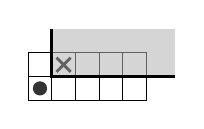
\begin{tikzpicture}[x=3mm,y=3mm,baseline=0pt]
\foreach \c in {1,...,5}{\draw[line width=.35pt] (\c-1,0) rectangle ++(1,1); \draw[line width=.35pt] (\c-1,1) rectangle ++(1,1);}
\fill[black!80] (.5,.5) circle (.3);
\draw[line width=1pt] (1.2,1.2) -- (1.8,1.8) (1.2,1.8) -- (1.8,1.2);
\fill[black!30,opacity=.55] (1,1) rectangle (6.2,3);
\draw[line width=1.2pt] (6.2,1) -- (1,1) -- (1,3);
\end{tikzpicture}\quad$\longrightarrow$\quad\bd[3]{5,1}{0}{0}{0}
\qquad{\small Step 2: input, card, output.}\par}

\textbf{A first hour.} After the five-minute movement opening and the five-minute launch, about 35--40 minutes at the tables and a few minutes to share one claim per table. Minutes beside each problem below are unpiloted estimates. First routes, with a core that ends the hour comfortably: \emph{K--1} Problems 1--3 (about 30 minutes), Problem 4 if time; \emph{grades 2--3} Problems 1--3 (about 35), with 4--5 as the continuation; \emph{grades 4--5} Problems 1--3 (about 30), with 4 as the continuation. Return visit: K--1 Problems 4--6; grades 2--3 Problems 4--6, 7 if ready; grades 4--5 Problems 5--6, where strategy stealing is the destination (4 first if not reached, 7 for whoever finishes). Finishing every page is not the goal.

\textbf{Hints only when needed.} ``What could your partner do next?'' ``Which board would you like to hand your partner?'' ``Did you try every bite?'' For a claimed rule, the adult plays against it.
\newpage
\head{Grades K--1: keys in plain words}
\textbf{The adult's strategies.} Do not suggest bites. When a child says ``I always win if I go here,'' play the other side as well as possible, like this. \emph{Two rows:} leave a board whose top row is one cookie shorter than the bottom row. On a full two-row board, eat the top-right cookie. Afterward, if the rows become equal, eat the top-right cookie; if the top row becomes two or more shorter, bite the bottom row so that it is one longer than the top. \emph{L shapes:} leave equal arms, then copy your partner's bite on the other arm. \emph{Squares:} eat the cookie diagonally next to the poison, which leaves equal arms, then copy.

\begin{center}
\begin{tabular}{@{}c@{\hspace{5mm}}c@{\hspace{5mm}}c@{\hspace{5mm}}c@{\hspace{5mm}}c@{}}
P1 & P2 & P3 & P4 & P5\\[2pt]
\bd[3]{2,1}{0}{0}{1}\ \bd[3]{2,2}{2}{2}{0}\ \bd[3]{3,1}{1}{3}{0} &
\bd[3]{3,3}{2}{3}{0}\ \bd[3]{4,4}{2}{4}{0} &
\bd[3]{3,1,1}{0}{0}{1}\ \bd[3]{4,1,1}{1}{4}{0} &
\bd[3]{3,3,3}{2}{2}{0}\ \bd[3]{4,4,4,4}{2}{2}{0} &
\bd[3]{6,6}{2}{6}{0}
\end{tabular}
\par\small Every X is the only winning first bite on its board, as is every winning bite in the later keys unless several are listed. Circled boards are wins for the player who goes second.
\end{center}

\sub[about 10 min]{Problem 1, page 1: three small boards}
Circle the first board (the poison, one cookie to its right and one above): whichever cookie you eat, your partner eats the other. On the second board X the top-right cookie; on the third, the far-right cookie. Each leaves your partner the circled shape. A child may say ``I give them the little corner.'' Hint: ``Which board on this page would you like your partner to have?''

\sub[10--15 min]{Problem 2, page 2: two rows}
Children may find the top-right bite by losing first: ``When I ate that one, my partner always won.'' Hint: ``What did your partner do just after your first bite?''

\sub[about 10 min]{Problem 3, page 3: L shapes}
Circle the first board (arms of 2 and 2). On the second (arms of 3 and 2) the first player eats the far-right cookie so the arms match. A child may explain with copying: ``Whatever you eat, I eat the same on my side.'' Hint: ``Is there anything different about the two boards?'' Follow-up: ``How do you know your partner can never win on the circled one?''

\sub[about 10 min]{Problem 4, page 4: squares}
The X leaves equal arms, the circled kind of board from Problem 3. Hint: ``Can you make a board from page 3?''

\sub[about 10 min]{Problem 5, page 5: 2~by~6}
As in Problem 2: eat the top-right cookie, then keep the top row one shorter.

\sub[15--20 min; build on the 4~by~4 board of page 4]{Problem 6, page 6: invent boards for the second player}
Inside 4~by~4 there are nine such boards with more than the poison, matching the nine grids; children may also offer the poison alone, which is correct. Check a colored grid against these pictures, each beside its flip:
\begin{center}
\bd[4]{2,1}{0}{0}{0}\hspace{3mm}\bd[4]{3,1,1}{0}{0}{0}\hspace{3mm}\bd[4]{4,1,1,1}{0}{0}{0}\hspace{7mm}
\bd[4]{3,2}{0}{0}{0}\hspace{3mm}\bd[4]{2,2,1}{0}{0}{0}\hspace{7mm}
\bd[4]{4,3}{0}{0}{0}\hspace{3mm}\bd[4]{2,2,2,1}{0}{0}{0}\hspace{7mm}
\bd[4]{4,2,2}{0}{0}{0}\hspace{3mm}\bd[4]{3,3,1,1}{0}{0}{0}\hspace{7mm}
\bd[4]{1}{0}{0}{0}
\end{center}
The first three are equal L shapes. The next two pairs each start with a two-row board whose top row is one shorter. A board is right if the second player keeps winning even when the first player tries hard. Hint: ``Can you use a board you circled?'' Extension: ``Turn your board so its rows become columns. Is it still a second-player board?''
\newpage
\head{Grades 2--3: rules found, then explained}
\sub[12--15 min; materials pp.\,2--3]{Problem 1, page 1: decide and explain}
In page order: \pos{3,1} bite $(1,3)$; \pos{2,1} none; \pos{2,2} bite $(2,2)$; \pos{3,2} none; \pos{4,2} bite $(1,4)$, leaving \pos{3,2}; \pos{3,1,1} none. For \pos{2,1}, either bite leaves one cookie for the partner to eat. For \pos{3,2}, each of the four bites has an answer: $(1,2)\to$ eat the top cookie; $(1,3)\to(2,2)$; $(2,1)\to(1,2)$; $(2,2)\to(1,3)$. Each answer leaves the poison alone or \pos{2,1}. For \pos{3,1,1}, copy on the other arm. ``I tried every bite and my partner always had an answer'' is a complete proof when every bite really was tried. Hint: ``How many different bites are there? Did you try them all?''

\sub[5--8 min; materials pp.\,1--2]{Problem 2, page 2: two-row rectangles}
The top-right cookie on $2\times3$, $2\times4$ and $2\times6$.

\sub[about 15 min; 2~by~6 board, \mat{1}]{Problem 3, page 2: the two-row rule}
\pos{5,4} none; \pos{5,2} $(1,4)$, leaving \pos{3,2}; \pos{5,3} $(1,5)$, leaving \pos{4,3}; \pos{4,1} $(1,3)$, leaving \pos{2,1}; \pos{6,5} none; \pos{6,3} $(1,5)$, leaving \pos{4,3}. \emph{Rule:} the player whose turn it is cannot make sure to win exactly when the top row is one shorter than the bottom row; the poison alone fits. \emph{Why:} the reply rule of Theorem 2. Hint: ``What is the same about the boards you could not win?'' Then: ``After your partner's bite, can you get back to a board like that?'' Follow-up: ``Does the rule work for one row?'' (Yes: top row 0.)

\sub[about 15 min; \mat{3}]{Problems 4--5, page 3: squares}
$(2,2)$ on $3\times3$ and $4\times4$. On $10\times10$, bite $(2,2)$, leaving arms of 9 and 9, then copy each bite on the other arm. After each of your turns the arms are equal, so your partner is the one who meets the poison alone. Follow-up: ``How do you know copying never runs out?''

\sub[10--15 min; 3~by~4 board, \mat{4}]{Problem 6, page 4: $3\times4$}
The only winning bite is $(2,3)$: middle row, third column, leaving \pos{4,2,2}. It is neither the top-right cookie nor the one next to the poison, so neither earlier trick applies. A child may try the top-right cookie first; the answer to it is $(2,3)$. \pos{4,2,2} loses for the player to move; each bite has an answer (bite $\to$ answer): $(1,2)\to(2,1)$, $(1,3)\to(3,2)$, $(1,4)\to(2,2)$ or $(3,1)$, $(2,1)\to(1,2)$, $(2,2)\to(1,4)$, $(3,1)\to(1,4)$, $(3,2)\to(1,3)$. Each answer leaves the poison alone, \pos{3,2}, \pos{2,2,1} or \pos{3,1,1}. Children can check a few of these against an adult rather than all. Hint: ``What happens if you use a trick that worked before?''

\sub[15--20 min; 3~by~5 board, \mat{4}]{Problem 7, page 5: three-row boards for the second player}
Exactly five fit in $3\times5$, so one grid stays empty:\hfill\raisebox{-2.6mm}{\bd[2.6]{2,2,1}{0}{0}{0}\hspace{5mm}\bd[2.6]{3,1,1}{0}{0}{0}\hspace{5mm}\bd[2.6]{4,2,2}{0}{0}{0}\hspace{5mm}\bd[2.6]{5,3,2}{0}{0}{0}\hspace{5mm}\bd[2.6]{5,5,3}{0}{0}{0}}\hspace*{\fill}\par
\pos{2,2,1} and \pos{3,1,1} appeared in Problem 1, and \pos{4,2,2} is Problem 6's answer. Two-row boards such as \pos{4,3} are correct second-player boards but do not have three rows. Pairs can pool their boards and test each other's by playing. Hint: ``Which board did your $3\times4$ bite leave?'' Readiness-dependent: $3\times7$ has five more, \pos{6,3,3}, \pos{6,4,2}, \pos{7,4,3}, \pos{7,5,2} and \pos{7,7,4}.

\head{Grades 4--5: from labels to a stolen strategy}
\sub[5--8 min; materials pp.\,1--3]{Problem 1, page 1: four rectangles}
$(2,4)$ on $2\times4$, $(2,6)$ on $2\times6$, $(2,2)$ on $3\times3$ and $4\times4$.

\sub[15--20 min; 3~by~3 board, \mat{3}]{Problem 2, page 2: every board inside $3\times3$}
By rows of the page: W W W W W; W W L L L; W W W W L; W W W L. The five L boards are \pos{3,2}, \pos{3,1,1}, \pos{2,2,1}, \pos{2,1} and the poison alone. Every winning bite on the W boards: \pos{3,3,3}, \pos{3,3,2} and \pos{2,2} bite $(2,2)$; \pos{3,3,1} bite $(1,3)$ or $(2,2)$; \pos{3,2,2} bite $(2,2)$ or $(3,1)$; \pos{3,2,1} bite $(1,3)$, $(2,2)$ or $(3,1)$; \pos{3,3} bite $(2,3)$; \pos{2,2,2} bite $(3,2)$; \pos{3,1} bite $(1,3)$; \pos{2,1,1} bite $(3,1)$; \pos{3} and \pos{2} bite $(1,2)$; \pos{1,1,1} and \pos{1,1} bite $(2,1)$. An L label needs every bite checked; a W label needs one bite. The page lists the biggest boards first, so working backward means starting at the end: label the last row together, then one child labels while another tests each label by playing, rotating. Hint: ``Which boards can you label without playing?''

\sub[5--8 min; 2~by~6 board, \mat{1}]{Problem 3, page 3: longer two-row boards}
\pos{5,4} none; \pos{6,3} $(1,5)$; \pos{4,1} $(1,3)$; \pos{6,5} none; \pos{5,2} $(1,4)$; \pos{6,4} $(1,6)$. Each winning bite leaves the top row one shorter.

\sub[10--15 min]{Problem 4, page 3: explanations for every size}
Two rows: eat the top-right cookie, then answer as in the overview, two cases. Squares bigger than one cookie: bite $(2,2)$, then copy. A full answer covers every kind of reply, not every reply. Hint: ``What kinds of bites can your partner make on a one-shorter board?''

\sub[about 20 min; 3~by~4 board, \mat{4}]{Problem 5, page 4: every winning first bite on $3\times4$}
Exactly one, $(2,3)$, leaving \pos{4,2,2}; the Grades 2--3 Problem 6 key above shows why that board loses. Every other bite has a refutation (bite $\to$ board $\to$ reply $\to$ board left):
\par\vspace{-1pt}{\centering\small\renewcommand{\arraystretch}{1.1}
\begin{tabular}{@{}l@{\hspace{10mm}}l@{}}
$(1,2)\to(1,1,1)\to(2,1)\to{}$poison alone & $(2,4)\to(4,3,3)\to(2,3)\to(4,2,2)$, or $(3,1)\to(4,3)$\\
$(1,3)\to(2,2,2)\to(3,2)\to(2,2,1)$ & $(3,1)\to(4,4)\to(2,4)\to(4,3)$\\
$(1,4)\to(3,3,3)\to(2,2)\to(3,1,1)$ & $(3,2)\to(4,4,1)\to(1,3)\to(2,2,1)$\\
$(2,1)\to(4)\to(1,2)\to{}$poison alone & $(3,3)\to(4,4,2)\to(2,3)\to(4,2,2)$\\
$(2,2)\to(4,1,1)\to(1,4)\to(3,1,1)$ & $(3,4)\to(4,4,3)\to(2,3)\to(4,2,2)$
\end{tabular}\par}
The twelve small grids are for this record; partners can split the eleven bites. Hint: ``For a bite you think fails, what would your partner do?'' Extension: $4\times5$ has only $(3,3)$.

\sub[15--20 min; 3~by~4 board, \mat{4}]{Problem 6, page 5: Ana's argument}
After the top-right bite the board is \pos{4,4,3}, and the second player's only winning reply is $(2,3)$, leaving \pos{4,2,2}. That is exactly the first player's own winning bite from Problem 5: the stolen move is visible. \emph{Ana is right.} Her argument is a proof by contradiction for every rectangle with more than one cookie, and it names no bite. (On $2\times n$ the top-right bite itself wins, so there is no winning reply to steal: the other case.) On \pos{3,1,1}, the step that breaks is ``every bite on the full board eats the top-right cookie too, so the first player could have made that same bite at the start.'' No cookie is in every bite: a bite on the right arm misses the top cookie, and the reverse. If the first player eats only the top cookie, the second player eats the end of the right arm, leaving arms of 1 and 1, a board no single first bite makes, since one bite shortens only one arm. ``It is not a rectangle'' is not yet the step; ask which sentence fails. Follow-up: ``Does Ana's argument tell you where to bite on $3\times5$?'' (No.)

\sub[about 15 min; \mat{4} and packet page 6]{Problem 7, page 6: three rows}
$3\times5$: $(3,4)$, leaving \pos{5,5,3}. $3\times6$: $(2,4)$, leaving \pos{6,3,3}. Test a candidate by finding the reply to every bite, or by playing an adult. Hint: ``Which three-row boards lose for the player to move? Can one bite leave one?'' For adults: $3\times7$ is $(3,5)$, $3\times8$ is $(2,5)$, and the tempting pattern then fails at $3\times9$ (overview).

\head{Sources and evidence}
{\small David Gale, ``A curious Nim-type game,'' \emph{American Mathematical Monthly} 81 (1974), 876--879: the game and strategy stealing. Berlekamp, Conway and Guy, \emph{Winning Ways for Your Mathematical Plays}, 2nd ed., on Chomp (chapter not checked). Doron Zeilberger, ``Three-rowed CHOMP,'' \emph{Advances in Applied Mathematics} 26 (2001): no simple three-row rule. JRMF, \emph{Chomp} (web page, accessed by the outline's author October 24, 2026; its activity guide is not in this checkout). None of these was consulted for this guide, and the JRMF page could not be reached from here. Every fact above was checked by computer against the final pages (script kept with the source); the general strategies rest on the proofs, not the computations. Library links: Week 7 (labeling by working backward), Week 8 and Week 1e (copying), Week 83 (valuing positions). The Hex draft also uses strategy stealing, so teach Chomp first. These pages are unpiloted. Record the preparation time, whether children remove exactly the cookies under the card, which problems each band reached, children's own explanations, and where an adult had to choose a bite.\par}
\end{document}
